\documentclass[11pt, a4paper]{article}
\usepackage[T2A]{fontenc}
\usepackage[utf8]{inputenc}
\usepackage[bulgarian, english]{babel}

%% Sets page size and margins
\usepackage[a4paper,top=3cm,bottom=3cm,left=3cm,right=3cm,marginparwidth=1.75cm]{geometry}

%% Useful packages
\usepackage{amsmath, amssymb, amsthm,calc,mathabx}
\usepackage{systeme}
\usepackage{graphicx}
\usepackage[colorinlistoftodos]{todonotes}
\usepackage[colorlinks=true, allcolors=black]{hyperref}
\usepackage{wrapfig,lipsum,booktabs}
\usepackage{enumitem}
\usepackage{float}
\usepackage{fmtcount}
\usepackage{multicol}
\usepackage{breqn}
\usepackage{setspace}
\usepackage{hyperref}
\usepackage {tikz}
	\usetikzlibrary {positioning}
	
\graphicspath{
	{Graphics/}
}

\newtheorem{theorem}{Theorem}

\newtheorem{lemma}{Lemma}
\newtheorem{prop}{Property}
\newtheorem*{remark}{Remark}

\theoremstyle{definition}
\newtheorem{definition}{Дефиниция}

\setlength{\columnsep}{1cm}
\setlength{\parindent}{1em}

\begin{document}
\begin{titlepage}
	\newcommand{\HRule}{\rule{\linewidth}{0.5mm}}
	\centering
	\textsc{\LARGE SRS 2019}\\[1cm]
	\HRule\\[1 cm]
	
	{\huge\bfseries Икономическо излседване на рансъмуер }\\[0.5 cm] 
	\HRule\\
    \vfill
			\Large
			\textit{Автор:}
			 \textsc{Никола Стайков}\\
             \vspace{2cm}
			\Large
			\textit{Ментор:}
            \textsc{Явор Папазов}
    \vfill	
	{\large\today}   
	\vfill
\end{titlepage}

\tableofcontents
\newpage
\begin{abstract}
		Ransomware е вид компютърен вирус, който критптира файловете на дадена система и изисква да бъде платен откуп, за да бъдат декриптирани. Приемаме, че създателите на Ransomware не знаят цената на данните на техните жертви, или по-точно колко техните жертви "мислят", че струват данните им. Те могат да правят малки проучвания преди да започнат основната кампания с цел да определят гореспоменатото разпределение. Този проект разглежда модел, чрез който да бъдат определени оптималните параметри за едно такова проучване. Този подход е ключов за намирането на оптималната цена за откупа.
\end{abstract}

\section{Introduction}
		Ransomware се появява за първи път през 1989 под формата на the AIDS Troyan, познат също като PC Cyborg.  The AIDS Trojan е бил доста лесен за преодоляване, тъй като използва симетрична криптография, и скоро са били разработени начини файловете да бъдат декриптирани, но този случай поставя началото на развитието на много от модерните заплахи. С навлизането на Интернет, ransomware се завръща с нова сили, а именно с the Archiveus Trojan и GPcode от 2006. Друг повратен момент в историята на malware е създаването на биткойн, и крипто-валутите като цяло, по много причини, някои от тях бидейки анонимността и автоматичните и невъзвръщаеми транзакции\cite{huang2018tracking}.\par
		В изминалите години е имало опити да бъде направен модел на пазара на malware. В \cite{caulfielddynamic}, авторите са създали теоретичен модел, взимайки предвид броя потребители, които имат backups, както и други фактори като разпространението на информация и надеждност на ransomware.           
		В \cite{cartwright2018pay} е изследван различен подход, който разглежда възможността за допълнително уговаряне на цената като игра между жертвата и престъпниците. Тази разработка се фокусира на теория на игрите и комбинаторика.\par
		Доста усилия са положени и за проследяването на плащания, свързани с ransomware в блокчейн, тъй като всички те са публични. В резултат на това има публични данни, свързани с тези плащания, предоставени от \cite{paquet2019ransomware} и в \cite{thomas2015framing} човек може да се запознае с много заключенияв, подкрепени с данни, отнасящи се не само до ransomware, но и до целия черен пазар.\par
		Моделът в настоящата разработка е базиран на описания в \cite{caulfielddynamic}, но се фокусира върху оптимизирането на параметри, които не са разгледани в споменатата статия.
\newpage
	\section{Preliminaries}
	В тази секция са включени всички дефиниции и концепции, които са нужни за цялостното разбиране на проекта.
		\begin{definition}
			\label{def:normdist}
			\emph{Normal Distribution}, означена  с $N(\mu, \sigma)$, е вид continuous distribution, където с $\mu$, $\sigma$ и $\sigma^{2}$ са означени среднoто аритметично, стандартната девиация и вариацията съответно.
		\end{definition}
	
		Графиката на тази функция образува крива, често наричана също камбанна крива. Тя има максимум $(x,f(x))$ в $\left(\mu, \dfrac{1}{\sigma\sqrt{2\pi}}\right)$:
		\begin{center}
			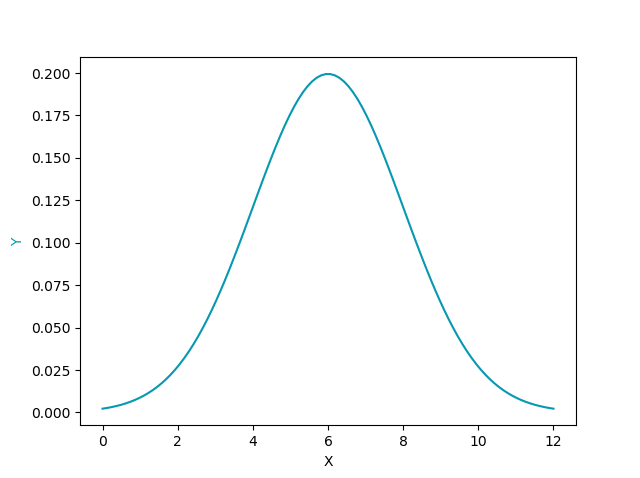
\includegraphics[width=0.6\textwidth]{Normal_clean}
		\end{center}
		
		\begin{definition}
			\label{def:def2}
			Consider a normal distribution $N(\mu, \sigma)$. \emph{Стандартната стойност}, или \emph{Z-score}, на дадено $x$ показва колко стандартни девиации е то от дадената средна стойност. Пресмята се по формулата $\dfrac{x-\mu}{\sigma}$.
		\end{definition}
	
		\begin{definition}
			\label{def:prob_dist}
			За дадено разпределение the \emph{probability distribution function} $F(x)$ показва вероятността стохастична променлива, следваща разпределението, да е по-малка или равна на $x$
			$$F_{X}(x)=\mathbb{P}(x\leq X).$$
		\end{definition}
	
		\begin{definition}
			\label{def:prob_dens}
			The \emph{Probability density function} на непрекъсната стохастична променлива $x$, описва вероятността дадена стохастична променлива $x$ да се окаже в произволен интервал. Формално се дефинира чрез
			\begin{align*}
				&\mathbb{P}(x < X \leq x+\Delta)=F_X(x+\Delta)-F_X(x)\\
				&f_X(x)=\lim_{\Delta \rightarrow 0} \frac{F_X(x+\Delta)-F_X(x)}{\Delta}.		
			\end{align*}
		\end{definition}
	
		\begin{definition}
			\label{def:err}
			\emph{The error function} е резултат на интегрирането на normal distribution, тя приема z-score като параметър и пресмята интеграла между фиксирана точка и средната стойност за разпределението.
			$$\operatorname{erf}(z)=\dfrac{2}{\sqrt{\pi}}\int_{0}^{z}e^{-t^{2}}dt.$$
		\end{definition}
	
	\section{Approach}
		Този модел описва разпространението на ransomware вирус. Намира оптималната цена на откуп за ransomware атака, която използва единствено botnets, без ключовия компонент на разпространяване на всеки компютър в мрежата. Този вариант на атаката е сравнително евтин за осъществяване, но има ниска ефективност. Третираме декриптирането на файловете на даден компютър като услуга, а откупа като нейната цена, съответно. \par
		Разглеждаме разпределението на Желанието за плащане (ЖЗП) на дадена тестова група. Това е максималната сума, която някой би платил за данните си. Поставяйки се в позицията на престъпниците се опитваме да открием разпределението чрез изследването на тестови групи от хора и как те реагират на дадена цена. Тези тестове обаче ни струват ценно време тъй като осведомеността на хората се показва постоянно. Искаме да разберем колко и колко големи тестове трябва да провеждаме, така че да направим модел на разпределението с приемлива грешка и в същото време без да губим твърде много време.\par
		За даден размер на тестовата група, изчисляваме грешката на дадена група от "потребители" от математически описаната функция на кривата на търсенето, която извличаме от разпределението на ЖЗП. Започвайки с малка група, постепенно увеличаваме размера на тестовата група, изчислявайки и грешката чрез метода на най-малките квадрати на всяка стъпка.
	\section{Model}
		Тук математическата страна на модела е разгледана подробно, показвайки как са достигнати резултатите и закюченията. Секцията е разделена на две смислови части, съответстващи на параметрите, които моделът изследва.
		\subsection{Sample size and error}
			Тази секция описва математическия модел, използвам за оптимизиране на грешката. Изведени са заключения относно размера на тестовата група.\par
			Приемаме, че стойността на данните на хората следва нормална дистрибуция и я свързваме със стохастичната променлива $p\sim N(500, 150)$. The probability density function (PDF) на нормална дистрибуция $N(\mu, \sigma)$ е $$\frac{1}{\sigma\sqrt{2\pi}}e^{-\frac{(x-\mu)^{2}}{2\sigma^{2}}}.$$\par\noindent
			За да изчислим функцията на търсене $f(k)$ от PDF за дадена цена $k$, трябва да изчислим
			$$\int_{k}^{\infty}f(x)\operatorname{d} x.$$
			\begin{figure}[H]
				\begin{minipage}{0.48\textwidth}
					\centering
					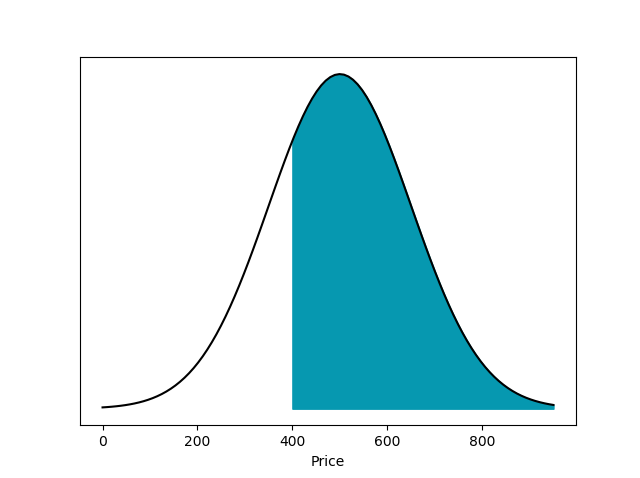
\includegraphics[width=\linewidth]{ND_integral}
					\caption{PDF}\label{Fig:Data1}
				\end{minipage}$\longrightarrow$
				\begin{minipage}{0.48\textwidth}
					\centering
					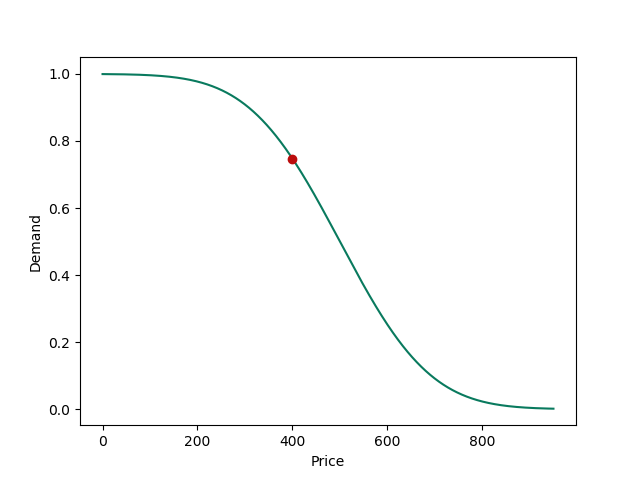
\includegraphics[width=\linewidth]{Sample_point}
					\caption{Price vs Demand}\label{Fig:Data2}
				\end{minipage}
			\end{figure}\par\noindent
			Отбелязаме, че интегралът трябва да бъде изчилсен до безкрайност, но след като $k$ стигне $\mu+3\sigma$, резултатът става пренебрежимо малък. Правейки това за цялата probability distribution function получаваме кривата на търсенето чрез процента хора, които биха платили. Нека означим кривата на търсенето с $F(x)$:
			$$
			F(x)=
			\begin{cases}
				\dfrac{1}{2}\left (1-\operatorname{erf}\left (\dfrac{z}{\sqrt{2}}\right )\right ) \text{if } x>\mu,\\
				\\
				\dfrac{1}{2}\left (1+\operatorname{erf}\left (\dfrac{z}{\sqrt{2}}\right )\right ) \text{if } x<\mu.
			\end{cases}
			$$\par
			Искаме да оптимизираме броя хора във всяка тестова група. Математическата функция, която искаме да опишем ни дава възможността да изчислим грешките от експерименталните данни с максимална точност.
			\begin{figure}[H]
				\begin{minipage}{0.48\textwidth}
					\centering
					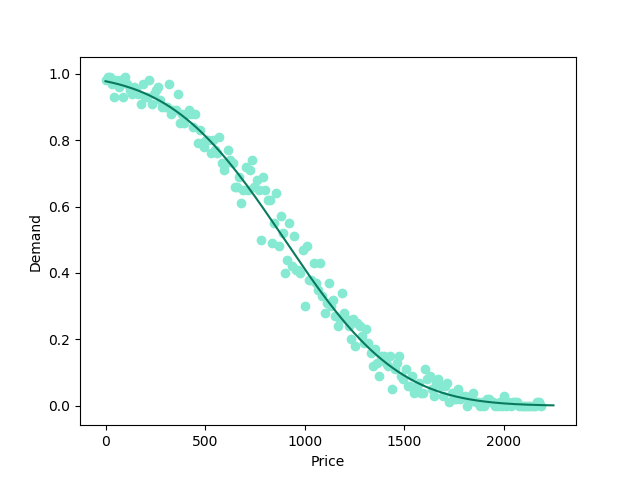
\includegraphics[width=\linewidth]{Exp_and_math_100}
					\caption{Sample size 100}\label{Fig:Data3}
				\end{minipage}\hfill
				\begin{minipage}{0.48\textwidth}
					\centering
					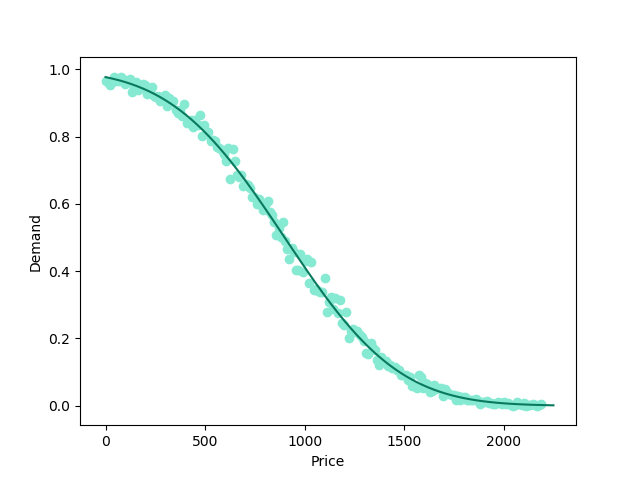
\includegraphics[width=\linewidth]{Exp_and_math_400}
					\caption{Sample size 400}\label{Fig:Data4}
				\end{minipage}
			\end{figure}\par\noindent
			Събирайки информация за размера на тестовата груап и грешките, съставяме графика, която показва тези промени.
			\begin{figure}[H]
			\begin{minipage}{1.0\textwidth}
				\centering
				\includegraphics[width=0.7\textwidth]{"Error vs sample size 4"}
				\caption{Тестов размер и грешка}\label{Fig:Data5}
			\end{minipage}
			\end{figure}
		\subsection{Backup function}
			В тази секция описваме функция, отговаряща за вероятността за присъствието на backup. Изчислен е ефектът и фърху очакваната печалба.\par
			Първо нека дефинираме the backup iterator $b$: 
			$$
			b=
			\begin{cases}
				1 \text{ if the victim has backup},\\
				0 \text{ if the victim does not have backup}
			\end{cases}
			$$
			Сега нека дефинираме желанието за плащане (ЖЗП):
			$$
			P(x)=
			\begin{cases}
			d_{x} \text{ if } b_{i}=0,\\
			c \text{ if } b_{i}=1
			\end{cases}
			$$
			Тук цената на backup е означена с $c$, а цената на данните на жертвата- с $d_{x}$.\par
			Както и по-рано, изчисляваме очакваната вероятност даден човек да плати цена $x$.
			Приемаме, че вероятността конкретна жертва да има backup е константа $p$ и изследваме как промяната на тази стойност влияе на очакваната печалба. Чрез събраните данни създаваме графика, която показва връзката между двете променливи.
			\begin{center}
				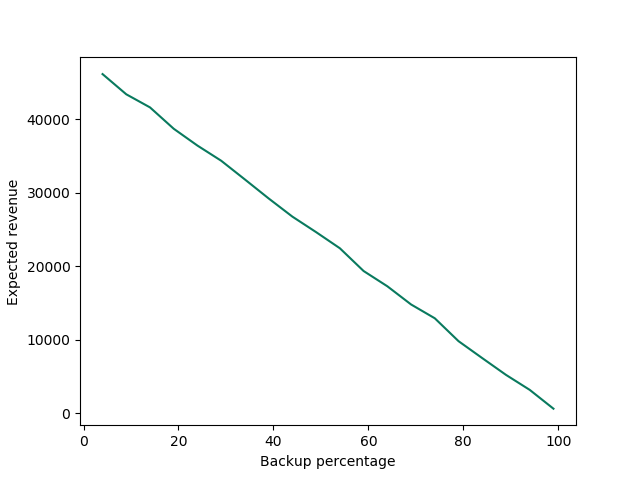
\includegraphics[width=0.55\textwidth]{Revenue_vs_backup}
			\end{center}
			
\section{Results}
	We have explored how the sample size affects the expected error between the statistical and experimental data and have explored how backups affect expected revenue. The model mainly focuses on optimizing the ransom prize, but the author truly believes that in order for us to be able to take countermeasures against ransomware attacks, we need to understand their every move. Putting ourselves in their shoes is essential to the purpose. Additional results, such as the distribution of expected revenue with respect to backup percentages, can help us to draw conclusions how to counteract.
\section{Further development}
	The author considers several future development directions for the project, namely:
	\begin{itemize}
		\item considering the use of backups and its influence on the WTP distribution
		\item expanding the model to describe more complex way of distributing the ransomware
		\item using the results and databases of related studies in order to back the project with real data\cite{paquet2019ransomware}
		\item considering a dynamic pricing model
	\end{itemize}
\section{Acknowledgments}
I want to thank my mentor, Yavor Papazov, and Konstantin Delchev for the enormous help with the choice of the research subject and for providing me with all the necessary material to get familiar with the topic, as well as listening to my questions along the whole way. I extend my gratitude towards Victor Velev, Victor Kolev and Stefan Hadzhistoikov for the support I got from them when I needed it the most. I also want to thank Stanislav Harizanov for the professional expertise.
\nocite{*}
\bibliographystyle{unsrt}
\bibliography{Bibliography}
\end{document}